%Afsnit 3 analyserer vi problemet (oversættelsen fra Hermes uden sidekanaler til ARM).
%Hvordan gør vi det egentlig, hvad skal vi være opmærksom på:
%Værktøjer vi bruger, hvorfor bruger vi dem, hvad skal vi gøre for at de kan bruges.
%Når afsnit 3 er færdig, så ved læseren hvad man skal gøre.
In our compilation from Hermes to ARM64 using Moscow ML\footnote{Moscow ML is a functional programming language widely used for teaching and research. More can be found at \url{http://www.itu.dk/~sestoft/mosml.html}}, we need to be aware of several things.

We are skipping some steps, as the current implementation is from Hermes to C and then to ARM.
But by skipping these steps, we have an easier time analyzing and optimizing. The question is how do we do it and what do we need to consider?

\section{Grammar}
In figure \ref{fig:hermes_grammar} the Hermes grammar is presented.
A Hermes Program consists of one or more Hermes Procedures each with an \bf{id}, a potentially empty list of declarations (function parameters) and a Hermes Block statement consisting of zero or more Hermes Stmts.
One of these Procedures must have the \bf{id} \emph{main} and take no arguments. This is the procedure that is first called when the program is executed.
Every procedure has to have exactly one Block statement. A Block is a special statement corresponding to a function body, consisting of a list of variable declarations followed by a list of Hermes Stmts.
Variable declarations (\emph{Decls1}) can be either variables, dynamic arrays or constants. Constants and constant arrays are public types and as so are not required to be zero at the end of a function. It is the responsibility of the programmer to make sure that sensitive information gets stored in the right variables.
Prior to this thesis Hermes only allowed constant declarations to be variables, but I've extended this to allow constant matrix declarations as well.
A ConstArrayDecl in the abstract syntax tree has the type \bf{string * string * string list * typ * pos} which is name, size, elements, type and position.
\begin{figure}[htp]
\centering
\begin{tabular}{>{$}l<{$}>{$}r<{$}>{$}l<{$}}
    Program   & \rightarrow & Procedure^+ \\[7pt]
    Procedure & \rightarrow & \textbf{id} \; ( \; Decls2^? \; ) \; Stmt \\[7pt]
    Stmt      & \rightarrow &; \\
              & |           & Lval \; \textbf{update} \; Exp \;; \\
              & |           & Lval\text{++} \;; \\
              & |           & Lval\text{- -} \;; \\
              & |           & \texttt{if} \; ( \; Exp \; ) \; Lval \; \textbf{update} \; Exp \;; \\
              & |           & Lval \; \text{<->} \; Lval \;; \\
              & |           & \texttt{if} \; ( \; Exp \; ) \; Lval \; \text{<->} \; Exp \;; \\
              & |           & \texttt{for} \; ( \; \textbf{id} = Exp \; ; \; Exp \; ) \; Stmt  \;; \\
              & |           & \texttt{assert} \; ( \; Exp \; ) \;; \\
              & |           & \texttt{call} \; \textbf{id} \; ( \; Lvals \; ) \;; \\
              & |           & \texttt{uncall} \; \textbf{id} \; ( \; Lvals \; ) \;; \\
              & |           & \texttt{printf} \; ( \; \textbf{stringConst} \; , \; Lvals \; ) \;; \\
              & |           & \texttt{scanf} \; ( \; \textbf{stringConst} \; , \; Lvals \; ) \;; \\
              & |           & \{ \; Decls1 \; Stmt^* \; \} \\[7pt]
    Exp       & \rightarrow & Lval \\
              & |           & \textbf{numConst} \; \\
              & |           & Exp \; \textbf{binOp} \; Exp \\
              & |           & \textbf{unOp} \; Exp \\
              & |           & ( \; Exp \; ) \; \\[7pt]
    Lval      & \rightarrow & \textbf{id}\\
              & |           & \textbf{id} \; [ \; Exp \; ] \\[7pt]
    Lvals     & \rightarrow & Lval \\
              & |           & Lval \; , \; Lvals \\[7pt]
    VarSpec   & \rightarrow & \textbf{id}\\
              & |           & \textbf{id} \; [ \; \textbf{numConst} \; ] \\[7pt]
    VarSpecs  & \rightarrow & VarSpec \\
              & |           & VarSpec \; , \; VarSpecs \\[7pt]
    Decls1    & \rightarrow & \\
              & |           & \textbf{type} \; Varspecs \; ; \; Decls1\\
              & |           & \texttt{const}\;\textbf{type}\;\textbf{id}\;=\textbf{numConst}\;;\;Decls1\;\\[7pt]
    Decls2    & \rightarrow & \textbf{type} \; VarSpec \\
              & |           &  \textbf{type} \; VarSpec \; , \; Decls2

\end{tabular}
\caption{Grammar of Hermes.}
\label{fig: grammar}
\end{figure}



\clearpage
\newpage

\section{Intermediate representations}
When compiling Hermes to RSSA, we use the procedure introduced in section \ref{section - RIL}.
We can do this in two iterations: first we translate to RIL, and then we translate to RSSA.
The reason for doing it in two steps is to postpone the problem of register allocation, and keep the two problems seperated.
We will be creating an abstract syntax tree that RIL and RSSA will share.
As seen in figure ~\ref{fig:RIL vs RSSA}, the main difference between the two representations is the subscript index on the left-values.
\begin{figure}[htp]
  \begin{center}
    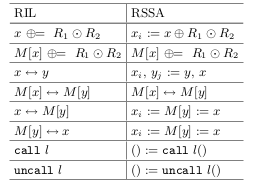
\includegraphics[width=0.6\textwidth]{RIL_RSSA_syntax.png}
  \end{center}
  \caption[caption]{RIL and RSSA syntax from\cite{10.1007/978-3-319-41579-6_16}}
  \label{fig:RIL vs RSSA}
\end{figure} \\
Variables that are going to have an index can be represented in SML as a tuple of a string variable name and an integer option index. The integer option can be NONE in the first iteration to RIL, and SOME int in the second iteration to RSSA. This makes it easy to seperate the two tasks and handle the indexing once the program has already been transformed to RIL.

Table \ref{table:translation} shows what RSSA statements different Hermes statements correspond to. Keep in mind that block, printf, scanf and assertion statements do not result in anything as they are only for debugging Hermes.
\begin{table}[htp]
  \begin{tabular}{| a | b |}
    \hline
    \rowcolor{LightCyan}
    \mc{1}{Hermes}      & \mc{1}{RSSA}                  \\ \hline
    Hermes.Skip         & RSSA.Skip                     \\
    Hermes.Update       & RSSA.Assign / RSSA.MemUpdate  \\
    Hermes.CondUpdate   & RSSA.If                       \\
    Hermes.Inc          & RSSA.Assign / RSSA.MemUpdate  \\
    Hermes.Dec          & RSSA.Assign / RSSA.MemUpdate  \\
    Hermes.Swap         & RSSA.AssignSwap / RSSA.MemSwap / RSSA.VarMemSwap \\
    Hermes.CondSwap     & RSSA.If with translated swap inside body \\
    Hermes.For          & RSSA.For  \\
    Hermes.Call         & RSSA.Call \\
    Hermes.Uncall       & RSSA.Uncall \\
    \hline
  \end{tabular}
  \caption{Translation table from Hermes to RSSA}
  \label{table:translation}
\end{table}
For the full details on how each Hermes Stmt is translated, see Appendix \ref{appendix:A}.

\section{Translation by hand}
%I afsnit 3 kan man vise hvordan man oversætter et Hermes program til RIL (det vi gjorde i hånden). Skal hjælpe læseren med at forstå nogle af de mere abstrakte begreber.
Lets have a look at a simple Hermes program and compile it by hand.
Usually it will be the programmers task to worry about values local to a function to be zero before the end of the function, but to make things simpler, we will omit this in the following translation example.
\lstinputlisting[label=listing:handtranslateHermes, caption=Simple Hermes program that does addition, language=Hermes, frame=single]{"Listings/handtranslateHermes.hms"}
After the parser and the lexer has run, the internal Hermes representation has the name of the function we are defining, "main", followed by a list of decls i.e. the function parameters.
Then comes the function body represented with a Block statement with local variable declarations "ds" and a list of statements corresponding to the \emph{++} and \emph{+=} statements in listing \ref{listing:handtranslateHermes}.
\lstinputlisting[label=listing:handtranslateHermesInternal, caption=Hermes internal representation of listing \ref{listing:handtranslateHermes}, language=Hermes, frame=single]{"Listings/handtranslateHermesInternal"}
When the RSSA compiler has run, the internal Hermes representation has been transformed into an internal RSSA representation containing references to variables and arrays etc.
As there are no RSSA statements for declaring variables, declarations are handled separately. They are translated to initialization- and finalization-strings in accordance with the RSSA standard from\cite{10.1007/978-3-319-41579-6_16} and inserted by the pretty-printer in case the target language is RIL or RSSA.
\lstinputlisting[label=listing:handtranslateRSSAInternal, caption=RSSA internal representation of listing \ref{listing:handtranslateHermes}, language=Hermes, frame=single]{"Listings/handtranslateRSSAInternal"}
When the ARM compiler has run, the internal RSSA representation has been transformed into an internal ARM representation.
\lstinputlisting[label=listing:handtranslateARMInternal, caption=ARM internal representation of listing \ref{listing:handtranslateHermes}, language=Hermes, frame=single]{"Listings/handtranslateARMInternal"}



%Oplagt at have et afsnit der beskriver de dele af ARM der er relevant i forhold til oversættelsen. Finder de instruktioner der er relevant. Hvad skal vi være opmærksomme på. Er der nogle vi ikke kan bruge fordi de generer sidekanaler? %TODO: det her afsnit skal skrives bedre
\section{Protection from side-channels}
One of the most difficult things of compilation is to protect against side-channel attacks. Hermes does an excellent job of promising that no sensitive information will be left in memory after execution, but how is this handled in our compilation to RSSA and ARM?
ARMs mult and div operations are very susceptible to power/timing attacks, and are (hopefully) avoided. Right now times and modulo uses mult. modulo also uses div. Its part of Hermes which means its really hard to avoid. But a lot of versions of ARM uses constant time multiplication. TODO: Expand on this.
Other side-channels such as power- and timing-attacks has to be dealt with in our ARM translation. % TODO: er det power eller timing med mult/div.


\section{Logical vs physical registers}
The ARM code that is produced by our compiler uses unbounded many abstract logical registers instead of actual physical registers.
It would require a register renaming before the code would actually be able to run on a device.
Register renaming is a technique that is used by high-performance processors to eliminate false data dependencies that can arise from the reuse of registers by successive instructions that do not have any real data dependencies between them.
The elimination of these false data dependencies can result in more instruction-level parallelism in a program, which can be exploited by techniques such as superscalar and out-of-order execution for better performance.
Register renaming or register allocation requires the creation of an inteference graph, which holds information about what values are \emph{simultaneously alive}. The graph is then colored using as few colors as possible. An example is shown in figure \ref{fig:interferencegraph} where we see that the same register could hold values a and b as they are not alive at the same time.

\begin{figure}[ht]
  \centering
  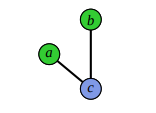
\includegraphics[scale=0.5]{Graphics/interferencegraph.png}
  \caption{An example of a coloured interference graph taken from \cite{ITU_liveness} }
  \label{fig:interferencegraph}
\end{figure}

In case there are too few registers/colours available to colour the interference graph, the excess values are \emph{spilled}, meaning that they are stored in memory instead.
